\section{Условие лабораторной работы}

Необходимо смоделировать систему, состоящую из генератора, памяти, и обслуживающего аппарата. 
Генератор подаёт сообщения, распределенные по равномерному закону, они приходят в память и выбираются на обработку по закону из ЛР2. 
Количество заявок конечно и задано. Предусмотреть случай, когда обработанная заявка возвращается обратно в очередь. 
Необходимо определить оптимальную длину очереди, при которой не будет потерянных сообщений. Реализовать двумя способами: используя пошаговый и событийный подходы

Распределение Пауссона (вариант 1)

\begin{figure}[h]
	\centering
	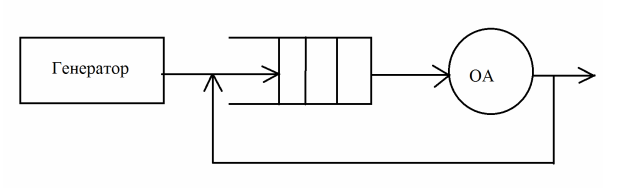
\includegraphics[width=0.7\linewidth]{src/CMO}
	\caption{}
	\label{fig:cmo}
\end{figure}
